\documentclass[11pt]{article}

    \usepackage[breakable]{tcolorbox}
    \usepackage{parskip} % Stop auto-indenting (to mimic markdown behaviour)
    
    \usepackage{iftex}
    \ifPDFTeX
    	\usepackage[T1]{fontenc}
    	\usepackage{mathpazo}
    \else
    	\usepackage{fontspec}
    \fi

    % Basic figure setup, for now with no caption control since it's done
    % automatically by Pandoc (which extracts ![](path) syntax from Markdown).
    \usepackage{graphicx}
    % Maintain compatibility with old templates. Remove in nbconvert 6.0
    \let\Oldincludegraphics\includegraphics
    % Ensure that by default, figures have no caption (until we provide a
    % proper Figure object with a Caption API and a way to capture that
    % in the conversion process - todo).
    \usepackage{caption}
    \DeclareCaptionFormat{nocaption}{}
    \captionsetup{format=nocaption,aboveskip=0pt,belowskip=0pt}

    \usepackage[Export]{adjustbox} % Used to constrain images to a maximum size
    \adjustboxset{max size={0.9\linewidth}{0.9\paperheight}}
    \usepackage{float}
    \floatplacement{figure}{H} % forces figures to be placed at the correct location
    \usepackage{xcolor} % Allow colors to be defined
    \usepackage{enumerate} % Needed for markdown enumerations to work
    \usepackage{geometry} % Used to adjust the document margins
    \usepackage{amsmath} % Equations
    \usepackage{amssymb} % Equations
    \usepackage{textcomp} % defines textquotesingle
    % Hack from http://tex.stackexchange.com/a/47451/13684:
    \AtBeginDocument{%
        \def\PYZsq{\textquotesingle}% Upright quotes in Pygmentized code
    }
    \usepackage{upquote} % Upright quotes for verbatim code
    \usepackage{eurosym} % defines \euro
    \usepackage[mathletters]{ucs} % Extended unicode (utf-8) support
    \usepackage{fancyvrb} % verbatim replacement that allows latex
    \usepackage{grffile} % extends the file name processing of package graphics 
                         % to support a larger range
    \makeatletter % fix for grffile with XeLaTeX
    \def\Gread@@xetex#1{%
      \IfFileExists{"\Gin@base".bb}%
      {\Gread@eps{\Gin@base.bb}}%
      {\Gread@@xetex@aux#1}%
    }
    \makeatother

    % The hyperref package gives us a pdf with properly built
    % internal navigation ('pdf bookmarks' for the table of contents,
    % internal cross-reference links, web links for URLs, etc.)
    \usepackage{hyperref}
    % The default LaTeX title has an obnoxious amount of whitespace. By default,
    % titling removes some of it. It also provides customization options.
    \usepackage{titling}
    \usepackage{longtable} % longtable support required by pandoc >1.10
    \usepackage{booktabs}  % table support for pandoc > 1.12.2
    \usepackage[inline]{enumitem} % IRkernel/repr support (it uses the enumerate* environment)
    \usepackage[normalem]{ulem} % ulem is needed to support strikethroughs (\sout)
                                % normalem makes italics be italics, not underlines
    \usepackage{mathrsfs}
    

    
    % Colors for the hyperref package
    \definecolor{urlcolor}{rgb}{0,.145,.698}
    \definecolor{linkcolor}{rgb}{.71,0.21,0.01}
    \definecolor{citecolor}{rgb}{.12,.54,.11}

    % ANSI colors
    \definecolor{ansi-black}{HTML}{3E424D}
    \definecolor{ansi-black-intense}{HTML}{282C36}
    \definecolor{ansi-red}{HTML}{E75C58}
    \definecolor{ansi-red-intense}{HTML}{B22B31}
    \definecolor{ansi-green}{HTML}{00A250}
    \definecolor{ansi-green-intense}{HTML}{007427}
    \definecolor{ansi-yellow}{HTML}{DDB62B}
    \definecolor{ansi-yellow-intense}{HTML}{B27D12}
    \definecolor{ansi-blue}{HTML}{208FFB}
    \definecolor{ansi-blue-intense}{HTML}{0065CA}
    \definecolor{ansi-magenta}{HTML}{D160C4}
    \definecolor{ansi-magenta-intense}{HTML}{A03196}
    \definecolor{ansi-cyan}{HTML}{60C6C8}
    \definecolor{ansi-cyan-intense}{HTML}{258F8F}
    \definecolor{ansi-white}{HTML}{C5C1B4}
    \definecolor{ansi-white-intense}{HTML}{A1A6B2}
    \definecolor{ansi-default-inverse-fg}{HTML}{FFFFFF}
    \definecolor{ansi-default-inverse-bg}{HTML}{000000}

    % commands and environments needed by pandoc snippets
    % extracted from the output of `pandoc -s`
    \providecommand{\tightlist}{%
      \setlength{\itemsep}{0pt}\setlength{\parskip}{0pt}}
    \DefineVerbatimEnvironment{Highlighting}{Verbatim}{commandchars=\\\{\}}
    % Add ',fontsize=\small' for more characters per line
    \newenvironment{Shaded}{}{}
    \newcommand{\KeywordTok}[1]{\textcolor[rgb]{0.00,0.44,0.13}{\textbf{{#1}}}}
    \newcommand{\DataTypeTok}[1]{\textcolor[rgb]{0.56,0.13,0.00}{{#1}}}
    \newcommand{\DecValTok}[1]{\textcolor[rgb]{0.25,0.63,0.44}{{#1}}}
    \newcommand{\BaseNTok}[1]{\textcolor[rgb]{0.25,0.63,0.44}{{#1}}}
    \newcommand{\FloatTok}[1]{\textcolor[rgb]{0.25,0.63,0.44}{{#1}}}
    \newcommand{\CharTok}[1]{\textcolor[rgb]{0.25,0.44,0.63}{{#1}}}
    \newcommand{\StringTok}[1]{\textcolor[rgb]{0.25,0.44,0.63}{{#1}}}
    \newcommand{\CommentTok}[1]{\textcolor[rgb]{0.38,0.63,0.69}{\textit{{#1}}}}
    \newcommand{\OtherTok}[1]{\textcolor[rgb]{0.00,0.44,0.13}{{#1}}}
    \newcommand{\AlertTok}[1]{\textcolor[rgb]{1.00,0.00,0.00}{\textbf{{#1}}}}
    \newcommand{\FunctionTok}[1]{\textcolor[rgb]{0.02,0.16,0.49}{{#1}}}
    \newcommand{\RegionMarkerTok}[1]{{#1}}
    \newcommand{\ErrorTok}[1]{\textcolor[rgb]{1.00,0.00,0.00}{\textbf{{#1}}}}
    \newcommand{\NormalTok}[1]{{#1}}
    
    % Additional commands for more recent versions of Pandoc
    \newcommand{\ConstantTok}[1]{\textcolor[rgb]{0.53,0.00,0.00}{{#1}}}
    \newcommand{\SpecialCharTok}[1]{\textcolor[rgb]{0.25,0.44,0.63}{{#1}}}
    \newcommand{\VerbatimStringTok}[1]{\textcolor[rgb]{0.25,0.44,0.63}{{#1}}}
    \newcommand{\SpecialStringTok}[1]{\textcolor[rgb]{0.73,0.40,0.53}{{#1}}}
    \newcommand{\ImportTok}[1]{{#1}}
    \newcommand{\DocumentationTok}[1]{\textcolor[rgb]{0.73,0.13,0.13}{\textit{{#1}}}}
    \newcommand{\AnnotationTok}[1]{\textcolor[rgb]{0.38,0.63,0.69}{\textbf{\textit{{#1}}}}}
    \newcommand{\CommentVarTok}[1]{\textcolor[rgb]{0.38,0.63,0.69}{\textbf{\textit{{#1}}}}}
    \newcommand{\VariableTok}[1]{\textcolor[rgb]{0.10,0.09,0.49}{{#1}}}
    \newcommand{\ControlFlowTok}[1]{\textcolor[rgb]{0.00,0.44,0.13}{\textbf{{#1}}}}
    \newcommand{\OperatorTok}[1]{\textcolor[rgb]{0.40,0.40,0.40}{{#1}}}
    \newcommand{\BuiltInTok}[1]{{#1}}
    \newcommand{\ExtensionTok}[1]{{#1}}
    \newcommand{\PreprocessorTok}[1]{\textcolor[rgb]{0.74,0.48,0.00}{{#1}}}
    \newcommand{\AttributeTok}[1]{\textcolor[rgb]{0.49,0.56,0.16}{{#1}}}
    \newcommand{\InformationTok}[1]{\textcolor[rgb]{0.38,0.63,0.69}{\textbf{\textit{{#1}}}}}
    \newcommand{\WarningTok}[1]{\textcolor[rgb]{0.38,0.63,0.69}{\textbf{\textit{{#1}}}}}
    
    
    % Define a nice break command that doesn't care if a line doesn't already
    % exist.
    \def\br{\hspace*{\fill} \\* }
    % Math Jax compatibility definitions
    \def\gt{>}
    \def\lt{<}
    \let\Oldtex\TeX
    \let\Oldlatex\LaTeX
    \renewcommand{\TeX}{\textrm{\Oldtex}}
    \renewcommand{\LaTeX}{\textrm{\Oldlatex}}
    % Document parameters
    % Document title
    \title{Tarea6\\M\'etodos Num\'ericos}
    \author{Benjamin Rivera}
    
    
    
    
    
% Pygments definitions
\makeatletter
\def\PY@reset{\let\PY@it=\relax \let\PY@bf=\relax%
    \let\PY@ul=\relax \let\PY@tc=\relax%
    \let\PY@bc=\relax \let\PY@ff=\relax}
\def\PY@tok#1{\csname PY@tok@#1\endcsname}
\def\PY@toks#1+{\ifx\relax#1\empty\else%
    \PY@tok{#1}\expandafter\PY@toks\fi}
\def\PY@do#1{\PY@bc{\PY@tc{\PY@ul{%
    \PY@it{\PY@bf{\PY@ff{#1}}}}}}}
\def\PY#1#2{\PY@reset\PY@toks#1+\relax+\PY@do{#2}}

\expandafter\def\csname PY@tok@w\endcsname{\def\PY@tc##1{\textcolor[rgb]{0.73,0.73,0.73}{##1}}}
\expandafter\def\csname PY@tok@c\endcsname{\let\PY@it=\textit\def\PY@tc##1{\textcolor[rgb]{0.25,0.50,0.50}{##1}}}
\expandafter\def\csname PY@tok@cp\endcsname{\def\PY@tc##1{\textcolor[rgb]{0.74,0.48,0.00}{##1}}}
\expandafter\def\csname PY@tok@k\endcsname{\let\PY@bf=\textbf\def\PY@tc##1{\textcolor[rgb]{0.00,0.50,0.00}{##1}}}
\expandafter\def\csname PY@tok@kp\endcsname{\def\PY@tc##1{\textcolor[rgb]{0.00,0.50,0.00}{##1}}}
\expandafter\def\csname PY@tok@kt\endcsname{\def\PY@tc##1{\textcolor[rgb]{0.69,0.00,0.25}{##1}}}
\expandafter\def\csname PY@tok@o\endcsname{\def\PY@tc##1{\textcolor[rgb]{0.40,0.40,0.40}{##1}}}
\expandafter\def\csname PY@tok@ow\endcsname{\let\PY@bf=\textbf\def\PY@tc##1{\textcolor[rgb]{0.67,0.13,1.00}{##1}}}
\expandafter\def\csname PY@tok@nb\endcsname{\def\PY@tc##1{\textcolor[rgb]{0.00,0.50,0.00}{##1}}}
\expandafter\def\csname PY@tok@nf\endcsname{\def\PY@tc##1{\textcolor[rgb]{0.00,0.00,1.00}{##1}}}
\expandafter\def\csname PY@tok@nc\endcsname{\let\PY@bf=\textbf\def\PY@tc##1{\textcolor[rgb]{0.00,0.00,1.00}{##1}}}
\expandafter\def\csname PY@tok@nn\endcsname{\let\PY@bf=\textbf\def\PY@tc##1{\textcolor[rgb]{0.00,0.00,1.00}{##1}}}
\expandafter\def\csname PY@tok@ne\endcsname{\let\PY@bf=\textbf\def\PY@tc##1{\textcolor[rgb]{0.82,0.25,0.23}{##1}}}
\expandafter\def\csname PY@tok@nv\endcsname{\def\PY@tc##1{\textcolor[rgb]{0.10,0.09,0.49}{##1}}}
\expandafter\def\csname PY@tok@no\endcsname{\def\PY@tc##1{\textcolor[rgb]{0.53,0.00,0.00}{##1}}}
\expandafter\def\csname PY@tok@nl\endcsname{\def\PY@tc##1{\textcolor[rgb]{0.63,0.63,0.00}{##1}}}
\expandafter\def\csname PY@tok@ni\endcsname{\let\PY@bf=\textbf\def\PY@tc##1{\textcolor[rgb]{0.60,0.60,0.60}{##1}}}
\expandafter\def\csname PY@tok@na\endcsname{\def\PY@tc##1{\textcolor[rgb]{0.49,0.56,0.16}{##1}}}
\expandafter\def\csname PY@tok@nt\endcsname{\let\PY@bf=\textbf\def\PY@tc##1{\textcolor[rgb]{0.00,0.50,0.00}{##1}}}
\expandafter\def\csname PY@tok@nd\endcsname{\def\PY@tc##1{\textcolor[rgb]{0.67,0.13,1.00}{##1}}}
\expandafter\def\csname PY@tok@s\endcsname{\def\PY@tc##1{\textcolor[rgb]{0.73,0.13,0.13}{##1}}}
\expandafter\def\csname PY@tok@sd\endcsname{\let\PY@it=\textit\def\PY@tc##1{\textcolor[rgb]{0.73,0.13,0.13}{##1}}}
\expandafter\def\csname PY@tok@si\endcsname{\let\PY@bf=\textbf\def\PY@tc##1{\textcolor[rgb]{0.73,0.40,0.53}{##1}}}
\expandafter\def\csname PY@tok@se\endcsname{\let\PY@bf=\textbf\def\PY@tc##1{\textcolor[rgb]{0.73,0.40,0.13}{##1}}}
\expandafter\def\csname PY@tok@sr\endcsname{\def\PY@tc##1{\textcolor[rgb]{0.73,0.40,0.53}{##1}}}
\expandafter\def\csname PY@tok@ss\endcsname{\def\PY@tc##1{\textcolor[rgb]{0.10,0.09,0.49}{##1}}}
\expandafter\def\csname PY@tok@sx\endcsname{\def\PY@tc##1{\textcolor[rgb]{0.00,0.50,0.00}{##1}}}
\expandafter\def\csname PY@tok@m\endcsname{\def\PY@tc##1{\textcolor[rgb]{0.40,0.40,0.40}{##1}}}
\expandafter\def\csname PY@tok@gh\endcsname{\let\PY@bf=\textbf\def\PY@tc##1{\textcolor[rgb]{0.00,0.00,0.50}{##1}}}
\expandafter\def\csname PY@tok@gu\endcsname{\let\PY@bf=\textbf\def\PY@tc##1{\textcolor[rgb]{0.50,0.00,0.50}{##1}}}
\expandafter\def\csname PY@tok@gd\endcsname{\def\PY@tc##1{\textcolor[rgb]{0.63,0.00,0.00}{##1}}}
\expandafter\def\csname PY@tok@gi\endcsname{\def\PY@tc##1{\textcolor[rgb]{0.00,0.63,0.00}{##1}}}
\expandafter\def\csname PY@tok@gr\endcsname{\def\PY@tc##1{\textcolor[rgb]{1.00,0.00,0.00}{##1}}}
\expandafter\def\csname PY@tok@ge\endcsname{\let\PY@it=\textit}
\expandafter\def\csname PY@tok@gs\endcsname{\let\PY@bf=\textbf}
\expandafter\def\csname PY@tok@gp\endcsname{\let\PY@bf=\textbf\def\PY@tc##1{\textcolor[rgb]{0.00,0.00,0.50}{##1}}}
\expandafter\def\csname PY@tok@go\endcsname{\def\PY@tc##1{\textcolor[rgb]{0.53,0.53,0.53}{##1}}}
\expandafter\def\csname PY@tok@gt\endcsname{\def\PY@tc##1{\textcolor[rgb]{0.00,0.27,0.87}{##1}}}
\expandafter\def\csname PY@tok@err\endcsname{\def\PY@bc##1{\setlength{\fboxsep}{0pt}\fcolorbox[rgb]{1.00,0.00,0.00}{1,1,1}{\strut ##1}}}
\expandafter\def\csname PY@tok@kc\endcsname{\let\PY@bf=\textbf\def\PY@tc##1{\textcolor[rgb]{0.00,0.50,0.00}{##1}}}
\expandafter\def\csname PY@tok@kd\endcsname{\let\PY@bf=\textbf\def\PY@tc##1{\textcolor[rgb]{0.00,0.50,0.00}{##1}}}
\expandafter\def\csname PY@tok@kn\endcsname{\let\PY@bf=\textbf\def\PY@tc##1{\textcolor[rgb]{0.00,0.50,0.00}{##1}}}
\expandafter\def\csname PY@tok@kr\endcsname{\let\PY@bf=\textbf\def\PY@tc##1{\textcolor[rgb]{0.00,0.50,0.00}{##1}}}
\expandafter\def\csname PY@tok@bp\endcsname{\def\PY@tc##1{\textcolor[rgb]{0.00,0.50,0.00}{##1}}}
\expandafter\def\csname PY@tok@fm\endcsname{\def\PY@tc##1{\textcolor[rgb]{0.00,0.00,1.00}{##1}}}
\expandafter\def\csname PY@tok@vc\endcsname{\def\PY@tc##1{\textcolor[rgb]{0.10,0.09,0.49}{##1}}}
\expandafter\def\csname PY@tok@vg\endcsname{\def\PY@tc##1{\textcolor[rgb]{0.10,0.09,0.49}{##1}}}
\expandafter\def\csname PY@tok@vi\endcsname{\def\PY@tc##1{\textcolor[rgb]{0.10,0.09,0.49}{##1}}}
\expandafter\def\csname PY@tok@vm\endcsname{\def\PY@tc##1{\textcolor[rgb]{0.10,0.09,0.49}{##1}}}
\expandafter\def\csname PY@tok@sa\endcsname{\def\PY@tc##1{\textcolor[rgb]{0.73,0.13,0.13}{##1}}}
\expandafter\def\csname PY@tok@sb\endcsname{\def\PY@tc##1{\textcolor[rgb]{0.73,0.13,0.13}{##1}}}
\expandafter\def\csname PY@tok@sc\endcsname{\def\PY@tc##1{\textcolor[rgb]{0.73,0.13,0.13}{##1}}}
\expandafter\def\csname PY@tok@dl\endcsname{\def\PY@tc##1{\textcolor[rgb]{0.73,0.13,0.13}{##1}}}
\expandafter\def\csname PY@tok@s2\endcsname{\def\PY@tc##1{\textcolor[rgb]{0.73,0.13,0.13}{##1}}}
\expandafter\def\csname PY@tok@sh\endcsname{\def\PY@tc##1{\textcolor[rgb]{0.73,0.13,0.13}{##1}}}
\expandafter\def\csname PY@tok@s1\endcsname{\def\PY@tc##1{\textcolor[rgb]{0.73,0.13,0.13}{##1}}}
\expandafter\def\csname PY@tok@mb\endcsname{\def\PY@tc##1{\textcolor[rgb]{0.40,0.40,0.40}{##1}}}
\expandafter\def\csname PY@tok@mf\endcsname{\def\PY@tc##1{\textcolor[rgb]{0.40,0.40,0.40}{##1}}}
\expandafter\def\csname PY@tok@mh\endcsname{\def\PY@tc##1{\textcolor[rgb]{0.40,0.40,0.40}{##1}}}
\expandafter\def\csname PY@tok@mi\endcsname{\def\PY@tc##1{\textcolor[rgb]{0.40,0.40,0.40}{##1}}}
\expandafter\def\csname PY@tok@il\endcsname{\def\PY@tc##1{\textcolor[rgb]{0.40,0.40,0.40}{##1}}}
\expandafter\def\csname PY@tok@mo\endcsname{\def\PY@tc##1{\textcolor[rgb]{0.40,0.40,0.40}{##1}}}
\expandafter\def\csname PY@tok@ch\endcsname{\let\PY@it=\textit\def\PY@tc##1{\textcolor[rgb]{0.25,0.50,0.50}{##1}}}
\expandafter\def\csname PY@tok@cm\endcsname{\let\PY@it=\textit\def\PY@tc##1{\textcolor[rgb]{0.25,0.50,0.50}{##1}}}
\expandafter\def\csname PY@tok@cpf\endcsname{\let\PY@it=\textit\def\PY@tc##1{\textcolor[rgb]{0.25,0.50,0.50}{##1}}}
\expandafter\def\csname PY@tok@c1\endcsname{\let\PY@it=\textit\def\PY@tc##1{\textcolor[rgb]{0.25,0.50,0.50}{##1}}}
\expandafter\def\csname PY@tok@cs\endcsname{\let\PY@it=\textit\def\PY@tc##1{\textcolor[rgb]{0.25,0.50,0.50}{##1}}}

\def\PYZbs{\char`\\}
\def\PYZus{\char`\_}
\def\PYZob{\char`\{}
\def\PYZcb{\char`\}}
\def\PYZca{\char`\^}
\def\PYZam{\char`\&}
\def\PYZlt{\char`\<}
\def\PYZgt{\char`\>}
\def\PYZsh{\char`\#}
\def\PYZpc{\char`\%}
\def\PYZdl{\char`\$}
\def\PYZhy{\char`\-}
\def\PYZsq{\char`\'}
\def\PYZdq{\char`\"}
\def\PYZti{\char`\~}
% for compatibility with earlier versions
\def\PYZat{@}
\def\PYZlb{[}
\def\PYZrb{]}
\makeatother


    % For linebreaks inside Verbatim environment from package fancyvrb. 
    \makeatletter
        \newbox\Wrappedcontinuationbox 
        \newbox\Wrappedvisiblespacebox 
        \newcommand*\Wrappedvisiblespace {\textcolor{red}{\textvisiblespace}} 
        \newcommand*\Wrappedcontinuationsymbol {\textcolor{red}{\llap{\tiny$\m@th\hookrightarrow$}}} 
        \newcommand*\Wrappedcontinuationindent {3ex } 
        \newcommand*\Wrappedafterbreak {\kern\Wrappedcontinuationindent\copy\Wrappedcontinuationbox} 
        % Take advantage of the already applied Pygments mark-up to insert 
        % potential linebreaks for TeX processing. 
        %        {, <, #, %, $, ' and ": go to next line. 
        %        _, }, ^, &, >, - and ~: stay at end of broken line. 
        % Use of \textquotesingle for straight quote. 
        \newcommand*\Wrappedbreaksatspecials {% 
            \def\PYGZus{\discretionary{\char`\_}{\Wrappedafterbreak}{\char`\_}}% 
            \def\PYGZob{\discretionary{}{\Wrappedafterbreak\char`\{}{\char`\{}}% 
            \def\PYGZcb{\discretionary{\char`\}}{\Wrappedafterbreak}{\char`\}}}% 
            \def\PYGZca{\discretionary{\char`\^}{\Wrappedafterbreak}{\char`\^}}% 
            \def\PYGZam{\discretionary{\char`\&}{\Wrappedafterbreak}{\char`\&}}% 
            \def\PYGZlt{\discretionary{}{\Wrappedafterbreak\char`\<}{\char`\<}}% 
            \def\PYGZgt{\discretionary{\char`\>}{\Wrappedafterbreak}{\char`\>}}% 
            \def\PYGZsh{\discretionary{}{\Wrappedafterbreak\char`\#}{\char`\#}}% 
            \def\PYGZpc{\discretionary{}{\Wrappedafterbreak\char`\%}{\char`\%}}% 
            \def\PYGZdl{\discretionary{}{\Wrappedafterbreak\char`\$}{\char`\$}}% 
            \def\PYGZhy{\discretionary{\char`\-}{\Wrappedafterbreak}{\char`\-}}% 
            \def\PYGZsq{\discretionary{}{\Wrappedafterbreak\textquotesingle}{\textquotesingle}}% 
            \def\PYGZdq{\discretionary{}{\Wrappedafterbreak\char`\"}{\char`\"}}% 
            \def\PYGZti{\discretionary{\char`\~}{\Wrappedafterbreak}{\char`\~}}% 
        } 
        % Some characters . , ; ? ! / are not pygmentized. 
        % This macro makes them "active" and they will insert potential linebreaks 
        \newcommand*\Wrappedbreaksatpunct {% 
            \lccode`\~`\.\lowercase{\def~}{\discretionary{\hbox{\char`\.}}{\Wrappedafterbreak}{\hbox{\char`\.}}}% 
            \lccode`\~`\,\lowercase{\def~}{\discretionary{\hbox{\char`\,}}{\Wrappedafterbreak}{\hbox{\char`\,}}}% 
            \lccode`\~`\;\lowercase{\def~}{\discretionary{\hbox{\char`\;}}{\Wrappedafterbreak}{\hbox{\char`\;}}}% 
            \lccode`\~`\:\lowercase{\def~}{\discretionary{\hbox{\char`\:}}{\Wrappedafterbreak}{\hbox{\char`\:}}}% 
            \lccode`\~`\?\lowercase{\def~}{\discretionary{\hbox{\char`\?}}{\Wrappedafterbreak}{\hbox{\char`\?}}}% 
            \lccode`\~`\!\lowercase{\def~}{\discretionary{\hbox{\char`\!}}{\Wrappedafterbreak}{\hbox{\char`\!}}}% 
            \lccode`\~`\/\lowercase{\def~}{\discretionary{\hbox{\char`\/}}{\Wrappedafterbreak}{\hbox{\char`\/}}}% 
            \catcode`\.\active
            \catcode`\,\active 
            \catcode`\;\active
            \catcode`\:\active
            \catcode`\?\active
            \catcode`\!\active
            \catcode`\/\active 
            \lccode`\~`\~ 	
        }
    \makeatother

    \let\OriginalVerbatim=\Verbatim
    \makeatletter
    \renewcommand{\Verbatim}[1][1]{%
        %\parskip\z@skip
        \sbox\Wrappedcontinuationbox {\Wrappedcontinuationsymbol}%
        \sbox\Wrappedvisiblespacebox {\FV@SetupFont\Wrappedvisiblespace}%
        \def\FancyVerbFormatLine ##1{\hsize\linewidth
            \vtop{\raggedright\hyphenpenalty\z@\exhyphenpenalty\z@
                \doublehyphendemerits\z@\finalhyphendemerits\z@
                \strut ##1\strut}%
        }%
        % If the linebreak is at a space, the latter will be displayed as visible
        % space at end of first line, and a continuation symbol starts next line.
        % Stretch/shrink are however usually zero for typewriter font.
        \def\FV@Space {%
            \nobreak\hskip\z@ plus\fontdimen3\font minus\fontdimen4\font
            \discretionary{\copy\Wrappedvisiblespacebox}{\Wrappedafterbreak}
            {\kern\fontdimen2\font}%
        }%
        
        % Allow breaks at special characters using \PYG... macros.
        \Wrappedbreaksatspecials
        % Breaks at punctuation characters . , ; ? ! and / need catcode=\active 	
        \OriginalVerbatim[#1,codes*=\Wrappedbreaksatpunct]%
    }
    \makeatother

    % Exact colors from NB
    \definecolor{incolor}{HTML}{303F9F}
    \definecolor{outcolor}{HTML}{D84315}
    \definecolor{cellborder}{HTML}{CFCFCF}
    \definecolor{cellbackground}{HTML}{F7F7F7}
    
    % prompt
    \makeatletter
    \newcommand{\boxspacing}{\kern\kvtcb@left@rule\kern\kvtcb@boxsep}
    \makeatother
    \newcommand{\prompt}[4]{
        \ttfamily\llap{{\color{#2}[#3]:\hspace{3pt}#4}}\vspace{-\baselineskip}
    }
    

    
    % Prevent overflowing lines due to hard-to-break entities
    \sloppy 
    % Setup hyperref package
    \hypersetup{
      breaklinks=true,  % so long urls are correctly broken across lines
      colorlinks=true,
      urlcolor=urlcolor,
      linkcolor=linkcolor,
      citecolor=citecolor,
      }
    % Slightly bigger margins than the latex defaults
    
    \usepackage[spanish]{babel}
    \usepackage{multicol}
    
    
    \geometry{tmargin=0.5in, bmargin=0.7in, lmargin=0.45in, rmargin=2.5in}
    \graphicspath{{assets/}}

\begin{document}
    
    \maketitle
    \tableofcontents
    

    \hypertarget{tarea-6}{%
\section{Tarea 6}\label{tarea-6}}

\emph{Tarea 6} de \emph{Benjamín Rivera} para el curso de
\textbf{Métodos Numéricos} impartido por \emph{Joaquín Peña Acevedo}.
Fecha limite de entrega \textbf{11 de Octubre de 2020}.

    \begin{tcolorbox}[breakable, size=fbox, boxrule=1pt, pad at break*=1mm,colback=cellbackground, colframe=cellborder]
\prompt{In}{incolor}{72}{\boxspacing}
\begin{Verbatim}[commandchars=\\\{\}]
\PY{k+kn}{import} \PY{n+nn}{sys}
\PY{k+kn}{import} \PY{n+nn}{seaborn} \PY{k}{as} \PY{n+nn}{sns}
\PY{k+kn}{import} \PY{n+nn}{scipy}

\PY{k+kn}{import} \PY{n+nn}{numpy} \PY{k}{as} \PY{n+nn}{np}
\PY{k+kn}{import} \PY{n+nn}{matplotlib}\PY{n+nn}{.}\PY{n+nn}{pyplot} \PY{k}{as} \PY{n+nn}{plt}
\PY{k+kn}{from} \PY{n+nn}{scipy}\PY{n+nn}{.}\PY{n+nn}{linalg} \PY{k+kn}{import} \PY{n}{solve\PYZus{}triangular} \PY{c+c1}{\PYZsh{} Para backward y forward substitution}

\PY{k+kn}{from} \PY{n+nn}{local}\PY{n+nn}{.}\PY{n+nn}{utils} \PY{k+kn}{import} \PY{o}{*}
\PY{k+kn}{from} \PY{n+nn}{local}\PY{n+nn}{.}\PY{n+nn}{Tarea4} \PY{k+kn}{import} \PY{n}{solChol}

\PY{n}{NOTEBOOK} \PY{o}{=} \PY{k+kc}{True}
\end{Verbatim}
\end{tcolorbox}










\newpage
    \hypertarget{ejercicio-1}{%
\subsection{Ejercicio 1}\label{ejercicio-1}}


\par Estas funciones no son utilizadas en el resto del programa pero fue solicitada en los enunciados de la tarea. Por lo que las programe pero despu\'es use las que tiene implementada la librer\'ia de python \verb|numpy|.

    \begin{tcolorbox}[breakable, size=fbox, boxrule=1pt, pad at break*=1mm,colback=cellbackground, colframe=cellborder]
\prompt{In}{incolor}{}{\boxspacing}
\begin{Verbatim}[commandchars=\\\{\}]
\PY{c+c1}{\PYZsh{} Parte 1}
\PY{c+c1}{\PYZsh{} Matriz traspuesta}

{\PY{k}{def} traspuesta(A,/, dtype=np.float32):}
\PY{l+s+sd}{    \PYZdq{}\PYZdq{}\PYZdq{} Funcion que regresa la matriz traspuesta. \PYZdq{}\PYZdq{}\PYZdq{}}
{    sz = A.shape}
{    ret = np.zeros((sz[1], sz[0]),}
{                   dtype=dtype)}
{    }
{    \PY{k}{for} i \PY{k}{in} \PY{n+nf}{range}(sz[0]):}
        \PY{k}{for}{ j \PY{k}{in} \PY{n+nf}{range}(sz[1]):}
{            ret[j,i] = A[i,j]}
{            }
\PY{k}{     return}{ ret}

\PY{c+c1}{\PYZsh{} Parte 2}
\PY{c+c1}{\PYZsh{} Producto de matrices}

\PY{k}{def} \PY{n+nf}{prodMat}{(A, B,/, dtype=np.float32):}
{    szA = A.shape}
{    szB = B.shape}
{    }
{    if szA[1] == szB[0]:}
{        ret = np.zeros((szA[0], szB[1]), dtype=dtype)}
{        }
{        for i in range(szA[0]):}
{            for j in range(szB[1]):}
{                ret[i,j] = sum(A[i,k]*B[k,j] for k in range(szA[1]))}
{        \PY{k}{return} ret}
\PY{k}{    else:}
{        \PY{k}{raise} \PY{n+nf}{Exception}(\PYZdq{}No coinciden las dimensiones\PYZdq{})}

\end{Verbatim}
\end{tcolorbox}





\newpage
    \begin{tcolorbox}[breakable, size=fbox, boxrule=1pt, pad at break*=1mm,colback=cellbackground, colframe=cellborder]
\prompt{In}{incolor}{4}{\boxspacing}
\begin{Verbatim}[commandchars=\\\{\}]
\PY{c+c1}{\PYZsh{} Parte 3}
\PY{c+c1}{\PYZsh{} Solucion de minimos cuadrados}

\PY{k}{def} \PY{n+nf}{minimosCuadrados}\PY{p}{(}\PY{n}{A}\PY{p}{,} \PY{n}{b}\PY{p}{,}\PY{o}{/}\PY{p}{,} \PY{n}{dtype}\PY{o}{=}\PY{n}{np}\PY{o}{.}\PY{n}{float64}\PY{p}{)}\PY{p}{:}
    \PY{l+s+sd}{\PYZdq{}\PYZdq{}\PYZdq{} Funcion que calcula la solucion de minimos cuadrados.}
\PY{l+s+sd}{    }
\PY{l+s+sd}{    Funcion que calcula la solucion de minimos cuadrado. Para}
\PY{l+s+sd}{    esto se basa de funciones ya implementadas para calcular}
\PY{l+s+sd}{    A\PYZca{}t@A y A\PYZca{}tb, para luego calcular la solucion del sitema}
\PY{l+s+sd}{    A\PYZca{}t@Ax = A\PYZca{}tb con fact de Cholesky.}
\PY{l+s+sd}{    }
\PY{l+s+sd}{    La funcion devuelve la solucion del sistema x si se encontro}
\PY{l+s+sd}{    y None en caso de que no se haya encontrado.}
\PY{l+s+sd}{    }
\PY{l+s+sd}{    A pesar de que la funcion tambien pide que se pasen las}
\PY{l+s+sd}{    dimensiones de las matrices, la forma pythonica no lo }
\PY{l+s+sd}{    requiere; por lo que seran obtenidas dentro del metodo.}
\PY{l+s+sd}{    }
\PY{l+s+sd}{    Input:}
\PY{l+s+sd}{        A := apuntador a matriz A}
\PY{l+s+sd}{        b := apuntador a vector b}
\PY{l+s+sd}{        }
\PY{l+s+sd}{    Output:}
\PY{l+s+sd}{        x := si existen sus valors; None en otro caso}
\PY{l+s+sd}{    \PYZdq{}\PYZdq{}\PYZdq{}}
    \PY{n}{x} \PY{o}{=} \PY{n}{np}\PY{o}{.}\PY{n}{zeros}\PY{p}{(}\PY{p}{(}\PY{n}{A}\PY{o}{.}\PY{n}{shape}\PY{p}{[}\PY{l+m+mi}{0}\PY{p}{]}\PY{p}{,}\PY{l+m+mi}{1}\PY{p}{)}\PY{p}{)}
        
    \PY{n}{At} \PY{o}{=} \PY{n}{A}\PY{o}{.}\PY{n}{transpose}\PY{p}{(}\PY{p}{)}\PY{n+nd}{@A}
    \PY{n}{yt} \PY{o}{=} \PY{n}{A}\PY{o}{.}\PY{n}{transpose}\PY{p}{(}\PY{p}{)}\PY{o}{*}\PY{n}{b}
    
    \PY{k}{return} \PY{n}{solChol}\PY{p}{(}\PY{n}{At}\PY{p}{,} \PY{n}{At}\PY{o}{.}\PY{n}{shape}\PY{p}{[}\PY{l+m+mi}{0}\PY{p}{]}\PY{p}{,} \PY{n}{yt}\PY{p}{)}
\end{Verbatim}
\end{tcolorbox}






\newpage
    \begin{tcolorbox}[breakable, size=fbox, boxrule=1pt, pad at break*=1mm,colback=cellbackground, colframe=cellborder]
\prompt{In}{incolor}{23}{\boxspacing}
\begin{Verbatim}[commandchars=\\\{\}]
\PY{c+c1}{\PYZsh{} Parte 4}

\PY{k}{def} \PY{n+nf}{get2Dvec}\PY{p}{(}\PY{n}{path}\PY{p}{,}\PY{o}{/}\PY{p}{,} \PY{n}{dtype}\PY{o}{=}\PY{n}{np}\PY{o}{.}\PY{n}{float64}\PY{p}{,} \PY{n}{info}\PY{o}{=}\PY{k+kc}{True}\PY{p}{)}\PY{p}{:}
    \PY{l+s+sd}{\PYZdq{}\PYZdq{}\PYZdq{} Funcion para cargar vector 2D.}
\PY{l+s+sd}{    }
\PY{l+s+sd}{    Esta funcion tratara de cargar un vector 2D de unarchivo}
\PY{l+s+sd}{    de texto que tenga dos columnas (correspondientes a dos}
\PY{l+s+sd}{    vectores y separada por un espacio) con k filas (donde k}
\PY{l+s+sd}{    es el tamanio de los vectores que estan separados por \PYZbs{}n)}
\PY{l+s+sd}{    }
\PY{l+s+sd}{    Los datos los guardaremos en una instancia de np.matrix}
\PY{l+s+sd}{    }
\PY{l+s+sd}{    Input:}
\PY{l+s+sd}{        path := direccion del archivo para cargar los}
\PY{l+s+sd}{            vectores}
\PY{l+s+sd}{            }
\PY{l+s+sd}{        dtype := tipo de dato para usar}
\PY{l+s+sd}{        info := Indica si queremos extraer la informacion}
\PY{l+s+sd}{    Output:}
\PY{l+s+sd}{        (ret, info)}
\PY{l+s+sd}{        ret := np.matrix de (2,k)}
\PY{l+s+sd}{        info := Para evitar tener que hacer otro recorrido}
\PY{l+s+sd}{            sobre el arreglo se puede extraer informacion}
\PY{l+s+sd}{            en este recorrido}
\PY{l+s+sd}{            minx := El minimo valor de x}
\PY{l+s+sd}{            maxx := El maximo valor de x}
\PY{l+s+sd}{    \PYZdq{}\PYZdq{}\PYZdq{}}
    
    \PY{k}{try}\PY{p}{:}
        ...
        \PY{k}{if} \PY{n}{info}\PY{p}{:}
            \PY{k}{return} \PY{n}{np}\PY{o}{.}\PY{n}{matrix}\PY{p}{(}\PY{n}{ret}\PY{p}{,} \PY{n}{dtype}\PY{o}{=}\PY{n}{dtype}\PY{p}{)}\PY{p}{,} \PY{n}{ret\PYZus{}info}
        \PY{k}{else}\PY{p}{:}
            \PY{k}{return} \PY{n}{np}\PY{o}{.}\PY{n}{matrix}\PY{p}{(}\PY{n}{Ret}\PY{p}{,} \PY{n}{dtype}\PY{o}{=}\PY{n}{dtype}\PY{p}{)}
    \PY{k}{except}\PY{p}{:}
        \PY{k}{raise} \PY{n+ne}{Exception}\PY{p}{(}\PY{l+s+s2}{\PYZdq{}}\PY{l+s+s2}{Error al cargar el archivo}\PY{l+s+s2}{\PYZdq{}}\PY{p}{)}


\PY{k}{def} \PY{n+nf}{plot\PYZus{}ej1\PYZus{}1}\PY{p}{(}\PY{n}{x}\PY{p}{,} \PY{n}{y}\PY{p}{)}\PY{p}{:}
    \PY{l+s+sd}{\PYZdq{}\PYZdq{}\PYZdq{} Funcion 1 para graficar resultados. }
\PY{l+s+sd}{    }
\PY{l+s+sd}{    Esta funcion buscca graficar los datos recibidos para poder}
\PY{l+s+sd}{    tomar la mejor decision respecto al grado a utilizar en la}
\PY{l+s+sd}{    aproximacion a polinomios.}
\PY{l+s+sd}{    }
\PY{l+s+sd}{    Input:}
\PY{l+s+sd}{        x := Valores de cordenadas x}
\PY{l+s+sd}{        y := Valores de cordenadas y}
\PY{l+s+sd}{    \PYZdq{}\PYZdq{}\PYZdq{}}


\PY{k}{def} \PY{n+nf}{plot\PYZus{}ej1\PYZus{}2}\PY{p}{(}\PY{n}{x}\PY{p}{,} \PY{n}{y}\PY{p}{,} \PY{n}{f}\PY{p}{,} \PY{n}{rng}\PY{p}{)}\PY{p}{:}
    \PY{l+s+sd}{\PYZdq{}\PYZdq{}\PYZdq{} Funcion 2 para graficar resultados}
\PY{l+s+sd}{    }
\PY{l+s+sd}{    Esta funcion busca graficar los datos recibidos para mostrar}
\PY{l+s+sd}{    la posible eproximacion obtenida por el metodo.}
\PY{l+s+sd}{    Input:}
\PY{l+s+sd}{        x := Valores de cordenadas x}
\PY{l+s+sd}{        y := Valores de cordenadas y}
\PY{l+s+sd}{        f := Funcion polinomica obtenida}
\PY{l+s+sd}{        rng := particion del rango para graficar}
\PY{l+s+sd}{    \PYZdq{}\PYZdq{}\PYZdq{}}

\PY{k}{def} \PY{n+nf}{error\PYZus{}ej1}\PY{p}{(}\PY{n}{p}\PY{p}{,} \PY{n}{x}\PY{p}{,} \PY{n}{y}\PY{p}{)}\PY{p}{:}
    \PY{l+s+sd}{\PYZdq{}\PYZdq{}\PYZdq{} Funcion para calcular error del polinomio. \PYZdq{}\PYZdq{}\PYZdq{}}
    \PY{k}{return} \PY{n+nb}{sum}\PY{p}{(}\PY{p}{(}\PY{n}{p}\PY{p}{(}\PY{n}{x}\PY{p}{[}\PY{n}{i}\PY{p}{]}\PY{p}{)} \PY{o}{\PYZhy{}} \PY{n}{y}\PY{p}{[}\PY{n}{i}\PY{p}{]}\PY{p}{)}\PY{o}{*}\PY{o}{*}\PY{l+m+mi}{2} \PY{k}{for} \PY{n}{i} \PY{o+ow}{in} \PY{n+nb}{range}\PY{p}{(}\PY{n+nb}{len}\PY{p}{(}\PY{n}{x}\PY{p}{)}\PY{p}{)}\PY{p}{)} 
    
    
\PY{k}{def} \PY{n+nf}{Ejercicio1}\PY{p}{(}\PY{n}{d}\PY{p}{,} \PY{n}{n\PYZus{}tabla}\PY{p}{,} \PY{n}{n}\PY{p}{,}\PY{o}{/}\PY{p}{,}\PY{n}{path}\PY{o}{=}\PY{l+s+s1}{\PYZsq{}}\PY{l+s+s1}{datos/}\PY{l+s+s1}{\PYZsq{}}\PY{p}{,} \PY{n}{dtype}\PY{o}{=}\PY{n}{np}\PY{o}{.}\PY{n}{float64}\PY{p}{,} \PY{n}{plot}\PY{o}{=}\PY{k+kc}{True}\PY{p}{,} \PY{n}{prnt}\PY{o}{=}\PY{k+kc}{True}\PY{p}{,} \PY{n}{ask}\PY{o}{=}\PY{k+kc}{True}\PY{p}{)}\PY{p}{:}
    \PY{c+c1}{\PYZsh{} Cargar datos}
    \PY{n}{tabla}\PY{p}{,} \PY{n}{info} \PY{o}{=} \PY{n}{get2Dvec}\PY{p}{(}\PY{n}{path}\PY{o}{+}\PY{n}{n\PYZus{}tabla}\PY{p}{,} 
                           \PY{n}{dtype}\PY{o}{=}\PY{n}{dtype}\PY{p}{)}
    \PY{c+c1}{\PYZsh{} Valores obtenidos}
    \PY{n}{x} \PY{o}{=} \PY{n}{np}\PY{o}{.}\PY{n}{ravel}\PY{p}{(}\PY{n}{tabla}\PY{p}{[}\PY{l+m+mi}{0}\PY{p}{,}\PY{p}{:}\PY{p}{]}\PY{p}{)}
    \PY{n}{y} \PY{o}{=} \PY{n}{np}\PY{o}{.}\PY{n}{ravel}\PY{p}{(}\PY{n}{tabla}\PY{p}{[}\PY{l+m+mi}{1}\PY{p}{,}\PY{p}{:}\PY{p}{]}\PY{p}{)}
    \PY{n}{rng} \PY{o}{=} \PY{n}{np}\PY{o}{.}\PY{n}{linspace}\PY{p}{(}\PY{n}{info}\PY{p}{[}\PY{l+s+s1}{\PYZsq{}}\PY{l+s+s1}{minx}\PY{l+s+s1}{\PYZsq{}}\PY{p}{]}\PY{p}{,} \PY{n}{info}\PY{p}{[}\PY{l+s+s1}{\PYZsq{}}\PY{l+s+s1}{maxx}\PY{l+s+s1}{\PYZsq{}}\PY{p}{]}\PY{p}{,} \PY{n}{num}\PY{o}{=}\PY{n}{d}\PY{p}{)}
    
    \PY{k}{if} \PY{n}{plot} \PY{o+ow}{and} \PY{n}{ask}\PY{p}{:} 
        \PY{n}{plot\PYZus{}ej1\PYZus{}1}\PY{p}{(}\PY{n}{x}\PY{p}{,}\PY{n}{y}\PY{p}{)}
    
    \PY{n}{sz} \PY{o}{=} \PY{n+nb}{len}\PY{p}{(}\PY{n}{x}\PY{p}{)}
    \PY{k}{if} \PY{n}{n} \PY{o}{\PYZlt{}} \PY{n}{sz}\PY{p}{:}
        \PY{c+c1}{\PYZsh{} Crear matriz a}
        \PY{n}{A} \PY{o}{=} \PY{n}{np}\PY{o}{.}\PY{n}{ones}\PY{p}{(}\PY{p}{(}\PY{n}{sz}\PY{p}{,} \PY{n}{n}\PY{o}{+}\PY{l+m+mi}{1}\PY{p}{)}\PY{p}{,} 
                    \PY{n}{dtype}\PY{o}{=}\PY{n}{dtype}\PY{p}{)}
        \PY{k}{for} \PY{n}{i} \PY{o+ow}{in} \PY{n+nb}{range}\PY{p}{(}\PY{n}{n}\PY{p}{)}\PY{p}{:}
            \PY{n}{A}\PY{p}{[}\PY{p}{:}\PY{p}{,}\PY{n}{i}\PY{p}{]} \PY{o}{=} \PY{n}{np}\PY{o}{.}\PY{n}{power}\PY{p}{(}\PY{n}{tabla}\PY{p}{[}\PY{l+m+mi}{0}\PY{p}{,}\PY{p}{:}\PY{p}{]}\PY{p}{,} \PY{n}{n}\PY{o}{\PYZhy{}}\PY{n}{i}\PY{p}{)}
        \PY{c+c1}{\PYZsh{} vector y}
        \PY{n}{b} \PY{o}{=} \PY{n}{np}\PY{o}{.}\PY{n}{matrix}\PY{p}{(}\PY{n}{tabla}\PY{p}{[}\PY{l+m+mi}{1}\PY{p}{,}\PY{p}{:}\PY{p}{]}\PY{p}{)}\PY{o}{.}\PY{n}{transpose}\PY{p}{(}\PY{p}{)}

        \PY{n}{coef} \PY{o}{=} \PY{n}{minimosCuadrados}\PY{p}{(}\PY{n}{A}\PY{p}{,} \PY{n}{b}\PY{p}{)}
        \PY{n}{p} \PY{o}{=} \PY{n}{f\PYZus{}polinomio}\PY{p}{(}\PY{n}{coef}\PY{p}{)}
        \PY{n}{write2Dvec}\PY{p}{(}\PY{n}{path}\PY{o}{+}\PY{l+s+s1}{\PYZsq{}}\PY{l+s+s1}{resp\PYZhy{}}\PY{l+s+s1}{\PYZsq{}}\PY{o}{+}\PY{n}{n\PYZus{}tabla}\PY{p}{,} \PY{n}{x}\PY{p}{,} \PY{p}{[}\PY{n}{p}\PY{p}{(}\PY{n}{xi}\PY{p}{)} \PY{k}{for} \PY{n}{xi} \PY{o+ow}{in} \PY{n}{x}\PY{p}{]}\PY{p}{)}

    \PY{k}{else}\PY{p}{:}
        \PY{k}{raise} \PY{n+ne}{Exception}\PY{p}{(}\PY{l+s+s2}{\PYZdq{}}\PY{l+s+s2}{Sistema indeterminado}\PY{l+s+s2}{\PYZdq{}}\PY{p}{)}
\end{Verbatim}
\end{tcolorbox}





\newpage
    \hypertarget{conjunto-1}{%
\subsubsection{Conjunto 1}\label{conjunto-1}}

Claramente se puede apreciar una parabola, por eso mi primer intento fue
tratar de conseguir un polinomio de grado \(2\). Esto es dificil de
mejorar, dado la dispercion de los puntos, ademas con n's muy grandes
empeiza a sufrir de \emph{overfitting} y no mejora el error; esto se
puede apreciar en el segundo intento con \(n = 11\)

    \begin{tcolorbox}[breakable, size=fbox, boxrule=1pt, pad at break*=1mm,colback=cellbackground, colframe=cellborder]
\prompt{In}{incolor}{12}{\boxspacing}
\begin{Verbatim}[commandchars=\\\{\}]
\PY{c+c1}{\PYZsh{} Parte 5}
\PY{k}{if} \PY{n}{NOTEBOOK}\PY{p}{:}
    \PY{n}{Ejercicio1}\PY{p}{(}\PY{l+m+mi}{50}\PY{p}{,} \PY{l+s+s1}{\PYZsq{}}\PY{l+s+s1}{puntos2D\PYZus{}conjunto1.txt}\PY{l+s+s1}{\PYZsq{}}\PY{p}{,} \PY{l+m+mi}{2}\PY{p}{)}
\end{Verbatim}
\end{tcolorbox}

    \begin{center}
    \adjustimage{max size={0.9\linewidth}{0.9\paperheight}}{output_7_0.png}
    \end{center}
    { \hspace*{\fill} \\}
    
    \begin{Verbatim}[commandchars=\\\{\}]
Seguro que quieres usar grado 2 para aproximar?
[S para mantener]: 2
n=2
    \end{Verbatim}

    \begin{center}
    \adjustimage{max size={0.9\linewidth}{0.9\paperheight}}{output_7_2.png}
    \end{center}
    { \hspace*{\fill} \\}
    
    \begin{Verbatim}[commandchars=\\\{\}]
Se encontraron los coeficientes
        0.7541817962086255, -10.231492940619027, 6.078939265117226
Error = 5650.301069137684
    \end{Verbatim}

    \begin{tcolorbox}[breakable, size=fbox, boxrule=1pt, pad at break*=1mm,colback=cellbackground, colframe=cellborder]
\prompt{In}{incolor}{32}{\boxspacing}
\begin{Verbatim}[commandchars=\\\{\}]
\PY{k}{if} \PY{n}{NOTEBOOK}\PY{p}{:}
    \PY{n}{Ejercicio1}\PY{p}{(}\PY{l+m+mi}{50}\PY{p}{,} \PY{l+s+s1}{\PYZsq{}}\PY{l+s+s1}{puntos2D\PYZus{}conjunto1.txt}\PY{l+s+s1}{\PYZsq{}}\PY{p}{,} \PY{l+m+mi}{11}\PY{p}{,} \PY{n}{ask}\PY{o}{=}\PY{k+kc}{False}\PY{p}{)}
\end{Verbatim}
\end{tcolorbox}

    \begin{center}
    \adjustimage{max size={0.9\linewidth}{0.9\paperheight}}{output_8_0.png}
    \end{center}
    { \hspace*{\fill} \\}
    
    \begin{Verbatim}[commandchars=\\\{\}]
Se encontraron los coeficientes
        -1.3588485818714197e-08, 1.2843215253923994e-06,
-5.2305115646995115e-05, 0.0012003310105050808, {\ldots}, -2.941809213167029,
-2.1452912757616205, -5.178739868339335, 7.361058552062617
Error = 5248.19300240789
    \end{Verbatim}

\subsubsection{Conjunto 2}

Respecto al conjunto dos lo primero que pense es que correspondia a una
funcion de grado 3, sin embargo el error queda bastante grande. En el
segundo intento pense que probablemente un polinomio de grado \(5\) se
ajustaria mejor, lo que mejoro considerablemente, ya que ahora el valor
es \(\sim 1\). En otros
intentos\footnote{Que no agregare a este reporte por ser muchos y muy a prueba y error}
vi que para bajar el error de \(0\) es necesario tomar un polinomio de
grado \(12\), que ya me parece que recolecta demasiada informacion que
podria no ser relevante.

    \begin{tcolorbox}[breakable, size=fbox, boxrule=1pt, pad at break*=1mm,colback=cellbackground, colframe=cellborder]
\prompt{In}{incolor}{16}{\boxspacing}
\begin{Verbatim}[commandchars=\\\{\}]
\PY{k}{if} \PY{n}{NOTEBOOK}\PY{p}{:}
    \PY{n}{Ejercicio1}\PY{p}{(}\PY{l+m+mi}{50}\PY{p}{,} \PY{l+s+s1}{\PYZsq{}}\PY{l+s+s1}{puntos2D\PYZus{}conjunto2.txt}\PY{l+s+s1}{\PYZsq{}}\PY{p}{,} \PY{l+m+mi}{3}\PY{p}{)}
\end{Verbatim}
\end{tcolorbox}

    \begin{center}
    \adjustimage{max size={0.9\linewidth}{0.9\paperheight}}{output_10_0.png}
    \end{center}
    { \hspace*{\fill} \\}
    
    \begin{Verbatim}[commandchars=\\\{\}]
Seguro que quieres usar grado 3 para aproximar?
[S para mantener]: s
n=3
    \end{Verbatim}

    \begin{center}
    \adjustimage{max size={0.9\linewidth}{0.9\paperheight}}{output_10_2.png}
    \end{center}
    { \hspace*{\fill} \\}
    
    \begin{Verbatim}[commandchars=\\\{\}]
Se encontraron los coeficientes
        -0.008095864120276854, 0.0030857409969524373, 0.347724224152898,
-0.04518101609383535
Error = 4.2437023557985745
    \end{Verbatim}

    \begin{tcolorbox}[breakable, size=fbox, boxrule=1pt, pad at break*=1mm,colback=cellbackground, colframe=cellborder]
\prompt{In}{incolor}{42}{\boxspacing}
\begin{Verbatim}[commandchars=\\\{\}]
\PY{k}{if} \PY{n}{NOTEBOOK}\PY{p}{:}
    \PY{n}{Ejercicio1}\PY{p}{(}\PY{l+m+mi}{50}\PY{p}{,} \PY{l+s+s1}{\PYZsq{}}\PY{l+s+s1}{puntos2D\PYZus{}conjunto2.txt}\PY{l+s+s1}{\PYZsq{}}\PY{p}{,} \PY{l+m+mi}{11}\PY{p}{,} \PY{n}{ask}\PY{o}{=}\PY{k+kc}{False}\PY{p}{)}
\end{Verbatim}
\end{tcolorbox}

    \begin{center}
    \adjustimage{max size={0.9\linewidth}{0.9\paperheight}}{output_11_0.png}
    \end{center}
    { \hspace*{\fill} \\}
    
    \begin{Verbatim}[commandchars=\\\{\}]
Se encontraron los coeficientes
        -1.5639735180840897e-09, -3.647711279013421e-09, 4.450736533289704e-07,
-1.7100043270209563e-06, {\ldots}, -0.022473411213090114, 0.01713626219890958,
0.49928235722555336, -0.0070410241304996795
Error = 1.0080196832546382
    \end{Verbatim}






\subsubsection{Conjunto 3}

Claramente podemos ver una distribucion normal en los puntos dispersos
que se muestran. El primer polinomio que tenia una apariencia similar a
esta fue el de grado \(4\), el cual daba un error \(\sim 2\). Despues de
eso la siguiente mejora considerable fue la del polinomio de grado
\(6\), que daba un error \(\sim 0.5\)

    \begin{tcolorbox}[breakable, size=fbox, boxrule=1pt, pad at break*=1mm,colback=cellbackground, colframe=cellborder]
\prompt{In}{incolor}{50}{\boxspacing}
\begin{Verbatim}[commandchars=\\\{\}]
\PY{k}{if} \PY{n}{NOTEBOOK}\PY{p}{:}
    \PY{n}{Ejercicio1}\PY{p}{(}\PY{l+m+mi}{50}\PY{p}{,} \PY{l+s+s1}{\PYZsq{}}\PY{l+s+s1}{puntos2D\PYZus{}conjunto3.txt}\PY{l+s+s1}{\PYZsq{}}\PY{p}{,} \PY{l+m+mi}{4}\PY{p}{,} \PY{n}{ask}\PY{o}{=}\PY{k+kc}{False}\PY{p}{)}
\end{Verbatim}
\end{tcolorbox}

    \begin{center}
    \adjustimage{max size={0.9\linewidth}{0.9\paperheight}}{output_13_0.png}
    \end{center}
    { \hspace*{\fill} \\}
    
    \begin{Verbatim}[commandchars=\\\{\}]
Se encontraron los coeficientes
        0.00032206033629311026, -0.0003855417565318806, -0.034690166313100616,
0.011550168869917873, 0.827944199634344
Error = 2.2603307586775965
    \end{Verbatim}

    \begin{tcolorbox}[breakable, size=fbox, boxrule=1pt, pad at break*=1mm,colback=cellbackground, colframe=cellborder]
\prompt{In}{incolor}{66}{\boxspacing}
\begin{Verbatim}[commandchars=\\\{\}]
\PY{k}{if} \PY{n}{NOTEBOOK}\PY{p}{:}
    \PY{n}{Ejercicio1}\PY{p}{(}\PY{l+m+mi}{50}\PY{p}{,} \PY{l+s+s1}{\PYZsq{}}\PY{l+s+s1}{puntos2D\PYZus{}conjunto3.txt}\PY{l+s+s1}{\PYZsq{}}\PY{p}{,} \PY{l+m+mi}{6}\PY{p}{,} \PY{n}{ask}\PY{o}{=}\PY{k+kc}{False}\PY{p}{)}
\end{Verbatim}
\end{tcolorbox}

    \begin{center}
    \adjustimage{max size={0.9\linewidth}{0.9\paperheight}}{output_14_0.png}
    \end{center}
    { \hspace*{\fill} \\}
    
    \begin{Verbatim}[commandchars=\\\{\}]
Se encontraron los coeficientes
        -7.065981612069293e-06, 9.045049435863039e-06, 0.0011564541100981907,
-0.000697767703063815, -0.059029633270661845, 0.008978629606807174,
0.9215749569687338
Error = 0.578133274637197
    \end{Verbatim}










\newpage
    \hypertarget{como-ejecutar}{%
\subsection{Como ejecutar}\label{como-ejecutar}}

\hypertarget{requerimientos}{%
\subparagraph{Requerimientos}\label{requerimientos}}

Este programa se ejecuto en mi computadora con la version de
\textbf{Python 3.8.2} y con estos
\href{https://github.com/BenchHPZ/UG-Compu/blob/master/MN/requerimientos.txt}{requerimientos}

\hypertarget{jupyter}{%
\paragraph{Jupyter}\label{jupyter}}

En caso de tener acceso a un \emph{servidor jupyter} ,con los
requerimientos antes mencionados, unicamente basta con ejecutar todas
las celdas de este \emph{notebook}. Probablemente no todas las celdas de
\emph{markdown} produzcan el mismo resultado por las
\href{jupyter-contrib-nbextensions.readthedocs.io}{\emph{Nbextensions}}.

\hypertarget{consola}{%
\paragraph{Consola}\label{consola}}

Habrá archivos e instrucciones para poder ejecutar cada uno de los
ejercicios desde la consola.

    \begin{tcolorbox}[breakable, size=fbox, boxrule=1pt, pad at break*=1mm,colback=cellbackground, colframe=cellborder]
\prompt{In}{incolor}{71}{\boxspacing}
\begin{Verbatim}[commandchars=\\\{\}]
\PY{n}{usage} \PY{o}{=} \PY{l+s+s2}{\PYZdq{}\PYZdq{}\PYZdq{}}
\PY{l+s+s2}{Programa correspondiente a la Tarea 6 de Metodos Numericos. }
\PY{l+s+s2}{Este programa espera leer los archivos de tipo npy}

\PY{l+s+s2}{Alumno: Benjamin Rivera}

\PY{l+s+s2}{Usage:}
\PY{l+s+s2}{  Tarea6.py ejercicio1 \PYZlt{}d\PYZgt{} \PYZlt{}tabla\PYZgt{} \PYZlt{}n\PYZgt{} [options]}
\PY{l+s+s2}{  Tarea6.py \PYZhy{}h | \PYZhy{}\PYZhy{}help}

\PY{l+s+s2}{Options:}
\PY{l+s+s2}{  \PYZhy{}\PYZhy{}path=\PYZlt{}path\PYZgt{}   Directorio para buscar archivos [default: datos/].}
\PY{l+s+s2}{  \PYZhy{}p \PYZhy{}\PYZhy{}nplot      Para no graficar los resultados}
\PY{l+s+s2}{  \PYZhy{}s \PYZhy{}\PYZhy{}nshow      Para no imprimir los resultados secundarios}
\PY{l+s+s2}{  \PYZhy{}a \PYZhy{}\PYZhy{}nask       Para no preguntar}
\PY{l+s+s2}{  \PYZhy{}h \PYZhy{}\PYZhy{}help       Show this screen.}
\PY{l+s+s2}{  \PYZhy{}v \PYZhy{}\PYZhy{}version    Show version.}
\PY{l+s+s2}{\PYZdq{}\PYZdq{}\PYZdq{}}

\end{Verbatim}
\end{tcolorbox}


    % Add a bibliography block to the postdoc
    
    
\begin{figure}[h]
	\centering
		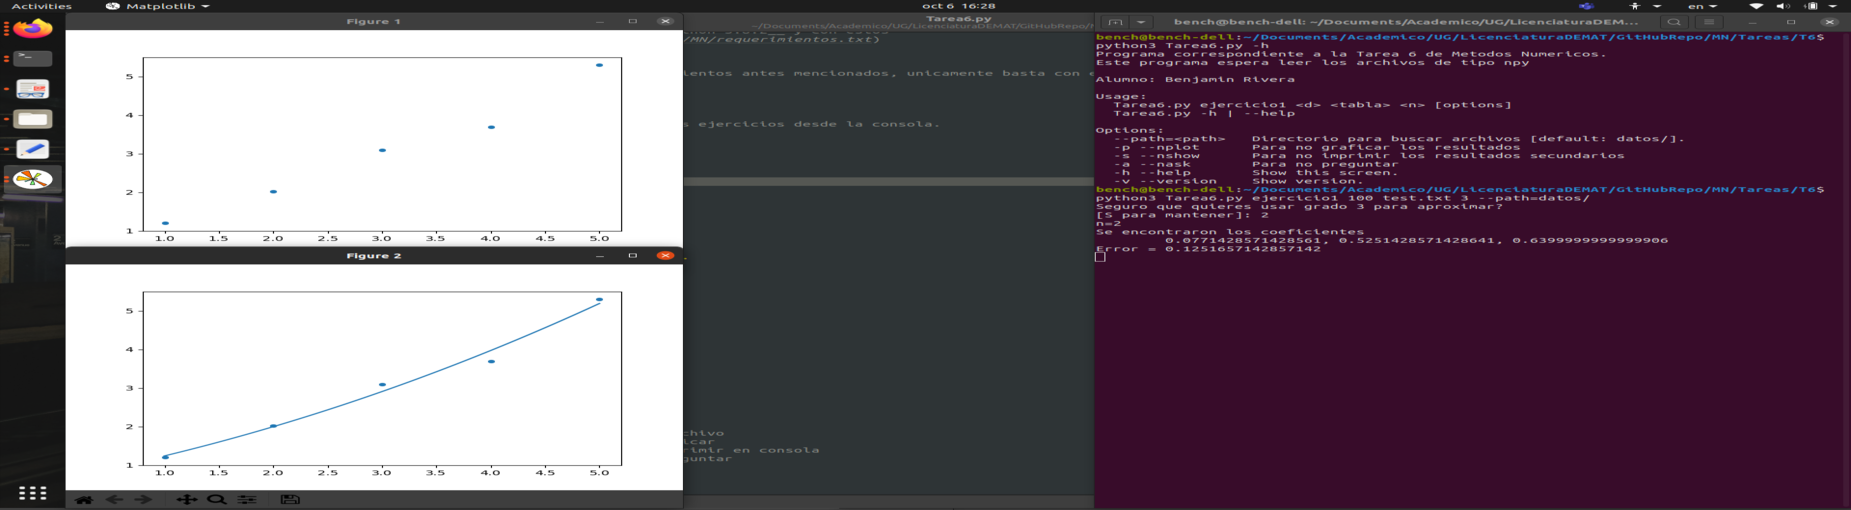
\includegraphics[width=1.0\textwidth]{trs.png}
	\caption{}
	\label{fig: ej1}
\end{figure}

\newpage

\begin{figure}[h]
	\centering
		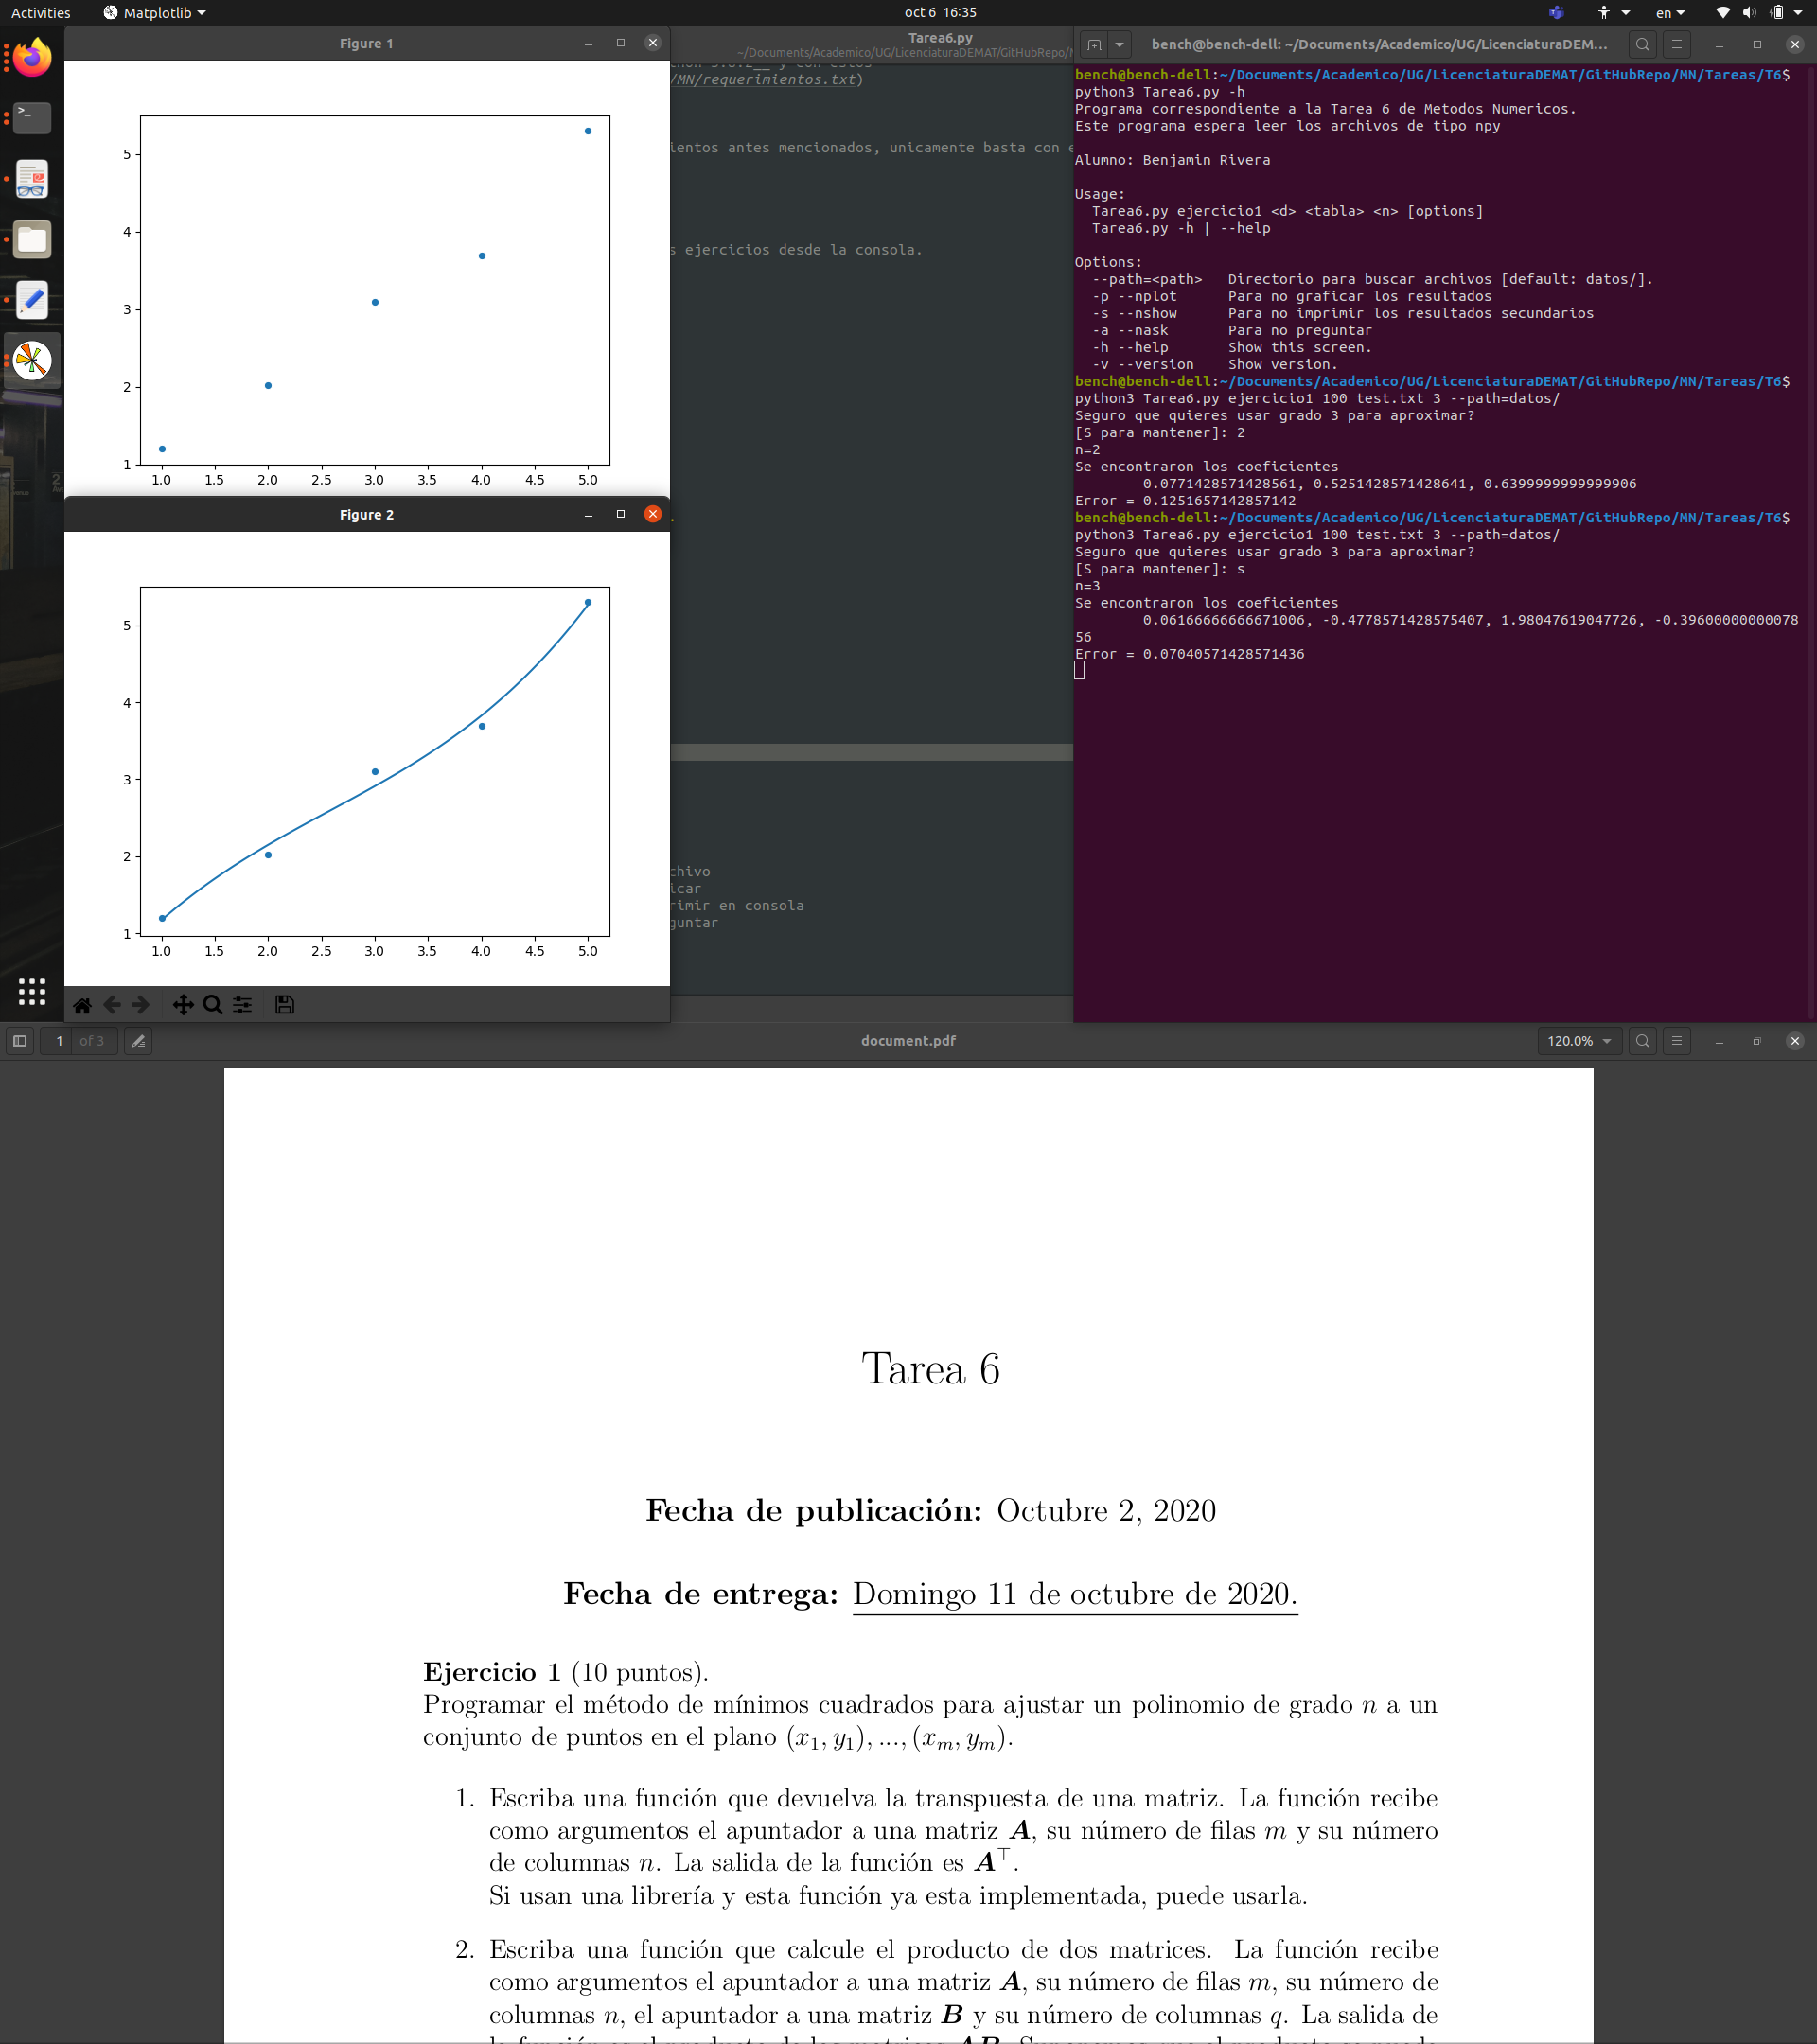
\includegraphics[width=1\textwidth]{trs2.png}
	\caption{Ejemplo de ejecucion del programa}
	\label{fig: ej2}
\end{figure}


    
    
    
\end{document}
